\documentclass{article}

\usepackage{amsmath}
\usepackage[dvips]{graphicx}

\usepackage{natbib}

\bibliographystyle{apa}

\begin{document}

\title{Solving for multi-class: a synthesis\\(manuscript in progress)}

\author{Peter Mills\\\textit{peteymills@hotmail.com}}

\maketitle

\section{Introduction}

\section{Definition of the problem}

\label{description}

In a statistical classication problem we are given a set of ordered pairs, 
$\lbrace \vec x_j : y_j \rbrace$ 
where $\vec x_j \in \Re^N$ is the location of the {\it sample} in 
the $N$-dimensional {\it feature space} 
and $y_j \in [1..n_c]$ is the class of the sample
where $n_c$ is the number of classes,
and the classes are
distributed according to an unknown conditional distribution,
$P(c | \vec x)$ with $c \in [1..n_c]$ the class label and $\vec x$ the location
in feature space.

Given an arbitrary {\it test point}, $\vec x$, 
we wish to estimate $P(c | \vec x)$, however we only have
the means to estimate some binary component of it, that is we have a 
set of binary classifiers, 
each returning a {\it decision function}, $r_i(\vec x)$.
In this paper we assume that the decision function 
returns estimates of the difference in conditional probabilities:
\begin{equation}
	r_i(\vec x) \approx p_i(+1|\vec x) - p_i(-1|\vec x)
\end{equation}
where $p_i(c|\vec x)$ is the conditional probability of the $i$th
binary classifier.
The decision function is trained using the same type of ordered pairs as
above except that the classes can only take on one of two values,
which for convenience are chosen as either $-1$ or $+1$, 
that is, $y_{ij} \in \lbrace -1, +1 \rbrace$.

How can we partition the classes, $\lbrace y_i \rbrace$, that is create
a mapping of the form:
\begin{equation}
	y_{ij} (y_j) = \left \lbrace  \begin{array}{lr}
-1 & | y_j \in C_i^+ \\
+1 & | y_j \in C_i^-
\end{array}
\right .
\end{equation}
where $y_{ij}$ is the class value of $j$th sample of the transformed data 
for trainng the $i$th binary classifier and 
$C_i^+ \subset [1,n_c]$ is the set of classes from the original set, 
$[1..n_c]$, that map to $+1$ while
$C_i^- \subset [1,n_c]$ is the set of classes that map to $-1$?

Once we have partitioned the classes
and trained the binary classifers,
how do we solve for the conditional probabilities, $P(i|\vec x)$,
where $i \in [1,n_c]$
or alternatively, directly for the most likely class:
%how do we solve for the most likely class, 
\begin{equation}
	c=\arg \max_i P(i | \vec x)
\end{equation}
?
%given a test point, $\vec x$,
%or alternatively, directly for $P(c | \vec x)$ where $c$ is either the most likely class
%or else can be any of the classes, $c \in [1,n_c]$?
%--that is all of the conditional probabilities 
%or just that of the ``winning'' class?

\section{Nonhierarchical multi-class classification}

In {\it non-hierarchical} multi-class classification, we solve for the
classes or probabilities of the multi-class problem all at once:
all the binary classifiers are used in the solution and the result of
one binary classifier does not determine the use of any of the others.
Using the notation provided in Section \ref{description}, 
we can write a system of equations relating
the multi-class conditional probabilities to the decision
functions:
\begin{equation}
	r_i(\vec x) = \frac{\sum_{j=1}^{n_i^+} P(c_{ij}^+|\vec x) - \sum_{j=1}^{n_{i}^-} P(c_{ij}^-|\vec x)}{\sum_{j=1}^{n_i^-} P(c_{ij}^-|\vec x) + \sum_{j=1}^{n_i^+} P(c_{ij}^+|\vec x)}
	\label{decision_function}
\end{equation}
where 
$c_{ij}^- \in C_i^-$,
$c_{ij}^+ \in C_i^+$,
$n_i^-$ is the number of class labels on the negative side of
the $i$th partition,
and $n_i^+$ is the number of class labels on the positive side of
the $i$th partition

It's more natural to describe the problem using a
{\it coding matrix}, $A$, 
which is structured such that
$a_{ij} \in \lbrace -1, 0, 1 \rbrace$ where $i$ enumerates the binary classifier and
$j$ enumerates the class of the multi-class problem.
In other words, if $a_{ij}$ is $-1$/$+1$, we would assign each of the $j$th class
labels in the training data a value of $-1$/$+1$ when training the $i$th
binary classifier. If the value is $0$, the $j$th class label is excluded.

The non-zero elements of $A$ are:
\begin{eqnarray}
	a_{ic_{ik}^-} & = & -1 | ~k = [1..n_{c_i^-}]\\
a_{ic_{ik}^+} & = & +1 | ~k=[1..n_{c_i^+}]
\end{eqnarray}

%We can relate the multi-class probabilities to the output of the 
%binary classifiers as follows:
We can rewrite Equation (\ref{decision_function}) using the decision
matrix as follows:
\begin{equation}
	\frac{\sum_j a_{ij} p_j}{\sum_j |a_{ij}| p_j} = r_i
	\label{non_hier}
\end{equation}
where $\vec p$, is a vector of multi-class conditional probabilities, $p_i=P(i|\vec x)$.

Some rearrangement shows that
we can solve for the probabilities, $\vec p$, via matrix inversion:
\begin{eqnarray}
	Q \vec p & = & \vec r \label{basic_system}\\
	%q_{ij} & = & a_{ij} + \delta(a_{ij}) r_i \\
	q_{ij} & = & a_{ij} + (1-|a_{ij}|) r_i 
	\label{matrix_equation2}
\end{eqnarray}
where $\vec r=\lbrace r_i| i=[1..n_p]\rbrace$ 
is the vector of decision functions, 
$n_p$ is the number of partitions,
$\vec p =\lbrace p_i | i=[1..n_c]\rbrace$
is the vector of estimated probabilities.
%and $\delta$ is the Kronecker delta.
Note that $Q$ reduces to $A$ if $A$ contains no zeroes.
The case of a coding matrix that contains no zeroes, that is all the partitions divide up all the
classes rather than a subset, will be called the {\it strict} case.
From a computational perspective, 
$Q$ must be regenerated for every new test point or value of $\vec r$ 
whereas $A$ can be inverted or decomposed and then
applied to every subsequent value of $\vec r$.

Because the decision functions, $\vec r$, are not estimated perfectly,
the final probabilities may need to be constrained and the inverse
problem solved via minimization:
\begin{equation}
	\vec p = \arg \min_{\vec v} | Q \vec v - \vec r | \label{minimization_problem}
\end{equation}
subject to:
\begin{eqnarray}
	\sum_{i=1}^{n_c} p_i & = & 1 \label{first_constraint}\\
	p_i & \ge & 0 \label{constraints}
\end{eqnarray}
where straight brackets, $||$, denotes a vector norm which  
in this case is the Euclidian or $L^2$ norm.

The class of the test point is determined through maximum likelihood:
\begin{equation}
	c = \arg \max_i p_i
\end{equation}

\subsection{Basic inverse solution}

Equation (\ref{minimization_problem}) can be solved via the normal
equation:
\begin{equation}
	Q^T Q \vec p = Q^T \vec r
	\label{normal_equation}
\end{equation}
Because the binary probability estimates in $\vec r$ are rarely perfect, however,
in many cases the constraints in (\ref{first_constraint}) and (\ref{constraints}) will not be satisfied 
so for most applications the results will need to be adjusted, reducing accuracy.

It is straightforward to incorporate the normality constraint in (\ref{first_constraint}) into the problem. There are at least three ways to do this. The most
obvious is to reduce the dimensionality of the problem by one:
\begin{equation}
	p_k = 1 - \sum_{i|i \ne k} p_i
\end{equation}
We can now rewrite the elements of the matrix, $Q$:
\begin{equation}
	q_{ij} = a_{ij} - a_{ik} + (|a_{ij}|-|a_{ik}|)r_i | ~ j \ne k
\end{equation}
and the solution vector which we'll now call $\vec b$:
\begin{equation}
	b_i = r_i - a_{ik} + (|a_{ik}| - 1) r_i
\end{equation}
Replace $\vec r$ with $\vec b$ in Equation (\ref{minimization_problem}) or (\ref{normal_equation}).

A more symmetric method involves adding an extra variable similar to
a Lagrange multiplier:
\begin{equation}
	\begin{bmatrix}
		Q^T Q & \vec 1 \\
		\vec 1 & 0
	\end{bmatrix}
	\begin{bmatrix}
		\vec p\\
		\lambda
	\end{bmatrix}
	= [\vec r, 1]
\end{equation}
where $\lambda$ is the Lagrange multiplier and $\vec 1$ is a vector of all ones.

If the number of partitions is one less than the number of classes, $n_p=n_c-1$,
the normality constraint, (\ref{first_constraint}), can simply be added to the 
matrix equation in (\ref{matrix_equation2}) as a row of all ones in $Q$ and a one in an augmented $\vec r$:
\begin{eqnarray}
	q_{n_c+1,j} & = & 1 \\
	r_{n_c+1} & = & 1
\end{eqnarray}

Since they are inequality constraints, those in (\ref{constraints}) are
harder to enforce.
The exception being the one-versus-one configuration: so long as the normality
constraint is satisfied, the inequality constraints are also satisfied
\citep{Wu_etal2004}.
Methods of enforceing the inequality constraints, (\ref{constraints}), will
be left to a later section.

\subsection{Voting solution}

In many other texts \citep{Allwein_etal2000, Hsu_Lin2002, Dietterich_Bakiri1995},
the class of the test point is determined by how close $\vec r$
is to each of the columns in $A$:
\begin{equation}
	c = \arg \min_i |\vec a^{(i)} - \vec r|^2
\end{equation}
where $\vec a^{(i)}$ is the $i$th column of $A$.
For the norm, $||$, Hamming distance is
frequently used, which is the number of bits that must be changed
in a binary number in order for it to match another binary number.
This assumes that each decision function returns only one of two values: 
$r_i \in \lbrace -1, +1 \rbrace$.
If the coding matrix is strict, then:
\begin{equation}
	|\vec a^{(j)} - \vec r| = \sum_i \delta_{a_{ij} r_i}
\end{equation}
where $\delta$ is the Kronecker delta.
\citet{Allwein_etal2000} 
tailor the matric on the basis of the binary classifier used, each of which
will return a different type of continuous decision function 
(that doesn't represent the difference in conditional probabilities).

Here we are assuming that the decision functions return an approximation of the 
difference in conditional probabilities of the binary classifier, hence we will once again use a
Euclidian metric. Expanding:
\begin{equation}
	c = \arg \min_i \left [|\vec a^{(i)}|^2 - 2 \vec a^{(i)} \cdot \vec r + |\vec r|^2 \right ]
\end{equation}
The length of $\vec r$ is independent of $i$, hence it can be eliminated from the expression.
For the strict case, the length of each column will also be constant at $|\vec a^{(i)}|=\sqrt{n_p}$.
Even for the non-strict case, we would expect the column lengths to be close for typical coding 
matrices. The column lengths are equal in the one-versus-one case for instance.
Eliminating these two terms produces a {\it voting} solution:
\begin{equation}
	c = \arg \max A^T \vec r
\end{equation}
That is, if the sign of $r_i$ matches the $i$th element of the column, then a vote is cast 
in proportion to the size of $r_i$ for the class label corresponding to the column number.

A voting solution can be used for any coding matrix and 
is especially appropriate if each $r_i$ returns on $-1$ or $+1$.  
The LIBSVM libary, for instance, uses a one-versus-one arrangement with a voting
solution if probabilities are not required \citep{Chang_Lin2011}.
The disadvantage of a voting solution is
that it does not return estimates of the probabilities.

\subsection{Common coding matrices}

There are number of standard, symmetric coding matrices that are commonly used
to solve for multi-class.
These include ``one-versus-the-rest'', ``one-versus-one'',
as well as error-correcting coding matrices including orthogonal and
random matrices.
We discuss each of these in turn.

\subsubsection{One-versus-the-rest}

Common coding matrices include ``one-versus-the-rest'' in which
we take each class and train it against the rest of the
classes.
For $n_c=4$ it works out to:
\begin{equation}
A = 
\begin{bmatrix}
1 & -1 & -1 & -1 \\
-1 & 1 & -1 & -1 \\
-1 & -1 & 1 & -1 \\
-1 & -1 & -1 & 1
\end{bmatrix}
\end{equation}
or in the general case:
\begin{equation}
	a_{ij}=2 \delta_{ij}-1
\end{equation}
where $\delta$ is the Kronecker delta.

Probabilities for the one-versus-the-rest can be solved for directly by
simply writing out one side of the equation:
\begin{equation}
	p_i = (r_i + 1)/2
\end{equation}
The normalization constraint, (\ref{first_constraint}), can be enforced 
through the use of a Lagrange multiplier. See next section.

\subsubsection{One-versus-one}

In a ``one-versus-one'' solution, we train each class against
every other class. For $n_c=4$:
\begin{equation}
A = 
\begin{bmatrix}
-1 & 1 & 0 & 0 \\
-1 & 0 & 1 & 0 \\
-1 & 0 & 0 & 1 \\
0 & -1 & 1 & 0 \\
0 & -1 & 0 & 1 \\
0 & 0 & -1 & 1
\end{bmatrix}
\end{equation}
The one-versus-one solution is used in LIBSVM \citep{Chang_Lin2011}.

Consider the following rearrangement of (\ref{non_hier}):
\begin{eqnarray}
	Q \vec p & = & \vec 0 \\
	q_{ij} & = & a_{ij} - r_i |a_{ij}|
\end{eqnarray}
We can include the normalization constraint, (\ref{first_constraint}), via
a Lagrange multiplier:
\begin{equation}
	\min_{\vec p, \lambda} | Q \vec p + \lambda(\vec 1 \cdot \vec p - 1)|
\end{equation}
which produces the following linear system:
\begin{eqnarray}
	\sum_k q_{ki} q_{kj} p_j + \lambda & = & 0 \\
	\sum_j p_j & = & 1
\end{eqnarray}
With this solution for a 1-vs-1 coding matrix, it can be shown that the
inequality constraints in (\ref{constraints}) are always satisfied
\citep{Wu_etal2004}.

\citet{Hsu_Lin2002} find that the one-vs.-one method is more accurate
for support vector machines (SVM) than either
error-correcting codes or one-vs.-the-rest.

\subsubsection{Orthogonal coding matrix}

To maximize the accuracy of an error-correcting coding matrix, 
the distance between each of the columns, $| \vec a^{(i)} - \vec a^{(j)} |$, 
should be as large as possible \citep{Allwein_etal2000, Windeatt_Ghaderi2002}, 
where $\vec a^({i})$ is the $i$th column of the matrix $A$ and $i \ne j$. 
If we take the upright brackets once again to be a
Euclidian metric and assume that $A$ is ``strict'' then this 
reduces to minimizing the absolute value of the dot product,
$|\vec a^{(i)} \cdot \vec a^{(j)}|$.
The absolute value is used because a pair of columns that are the same except 
for a factor of -1 are degenerate.

In other words, 
%if the number of rows is equal to the number of classes, 
the optimal coding matrix will be orthogonal, $A^T A = n_p I$, where $I$ is
the identity matrix. Thus the voting solution and the (unconstrained) matrix 
inverse will be equivalent. Orthogonal, ``strict'' coding matrices 
are not hard to construct for certain class sizes, for instance:
\begin{equation}
A = 
\begin{bmatrix}
1 & -1 & -1 & -1 \\
-1 & 1 & 1 & 1 \\
-1 & -1 & -1 & 1 \\
-1 & -1 & 1 & -1
\end{bmatrix}
\end{equation}
Orthogonal coding matrices for the non-strict case are even easier to
construct, but the voting solution does not correspond to the inverse solution.

\citet{Mills2017} shows how to solve for an orthogonal coding matrix.

\subsubsection{Error correcting codes}

Another common coding matrix is simply a random one: this is commonly
known as an ``error-correcting'' code \citep{Dietterich_Bakiri1995}.
To solve for the probabilities using an arbitary coding matrices
we transform the problem to an equivalent problem with an orthogonal
matrix.
We wish to transform the problem as follows:
\begin{equation}
	V^\prime Q \vec p = V^\prime \vec r
\end{equation}
Consider the singular value decomposition of $Q$:
\begin{equation}
	Q Q^T U = S^2 U
\end{equation}
where $U$ is an $n_p \times n_c$ ortho-normal matrix and $S$ is a diagonal
matrix of singular values.
Hence:
\begin{equation}
	V^\prime = U^T S^{-1}
\end{equation}
and
\begin{equation}
	V^\prime Q = U^T S^{-1} Q = V
\end{equation}
where $V$ is other half of the singular value decomposition:
\begin{eqnarray}
	Q & = & U S V^T \\
	Q^T Q V & = & V S^2
\end{eqnarray}
Hence, the solution for orthogonal matrices generalizes to non-orthogonal, 
non-strict coding matrices by setting $p_0$ to the least-squares solution:
\begin{equation}
	\vec p_0 = V S^{-1} U^T \vec r
\end{equation}
or equivalently:
\begin{equation}
	Q^T Q \vec p_0 = Q^T \vec r
\end{equation}

[whut????]


\section{Decision trees}

The most obvious method of dividing up a multi-class problem into binary
classifiers is hierarchically using a {\it decision tree} 
\citep{Cheong_etal2004, Lee_Oh2003}.
In this method, the classes are first divided into two partitions, then
those partitions are each divided into two partitions and so on until only
one class remains. The classification scheme is hierarchical, with all the
losing classes being excluded from the consideration at each step.
Only the conditional probability of the winning class is calculated as the
product of all the returned conditional probabilities of the binary
classifiers.

Decision trees have the advantage that they are fast since on average they
require only $\log_2 n_c$ classifications and there is no need to solve a 
constrained matrix inverse. On the other hand, because there is less
information being taken into consideration, they also tend to be less
accurate [citation].

Interestingly, the same partitions created for a decision tree can also
be used in a non-hierarchical scheme
to solve for all of the conditional probabilities. Consider the following
coding matrix for instance:
\begin{equation}
A = 
\begin{bmatrix}
1 & 1 & -1 & -1 \\
-1 & 1 & 0 & 0 \\
0 & 0 & -1 & 1
\end{bmatrix}
\end{equation}
While there are only three rows for four classes, 
once we add in the constraint in (\ref{first_constraint}) the system becomes 
fully determined, although it doesn't scale to larger problems:
extra partitions will have to be added.

\subsection{Variations}

There are many variations on the method. \citet{Ramanan_etal2007} for instance train a 
one-versus-the-rest model at each level of the tree so that if the ``one''
class is returned, the lower levels of the tree are short circuited
and this class is selected for the final result. Otherwise, the one class
is left out of subsequent analysis. This is less a new method than simply
a means of shaping the tree appropriate to datasets with unbalanced
numbers of classes, for instance the ``Shuttle'' dataset \citep{King_etal1995}.

In a decision directed acyclic graph (DDAG), 
rather than testing one group against another, 
each node of the tree tests one class against another \citep{Platt_etal2000}. 
The losing class is excluded from subsequent analysis. 
The previous paragraph describes the ``tree'' version of the one-versus-the-rest. 
This is the tree version of one-versus-one. 
In a DDAG, there are multiple paths to the same node.

\subsection{Empirically designed trees}

\begin{figure}
	\includegraphics[width=0.9\textwidth]{landclasstree.eps}
	\label{landclasstree}
\end{figure}

Consider the following land-classification problem: you have remote-sensing measurements of four surface types: corn field, wheat field, evergreen forest and deciduous forest.
How do you divide up the tree to best classify the measurements into one of these four surface types?
A priori, it would make the most sense to first divide them by their more general grouping: field versus forest and then, once you have field, classify by type of field, or if you have forest, classify by the type of forest.
This is illustrated in Figure \ref{landclasstree}.

In this case we have prior knowledge of how the classes are related to one another,
but in many cases, we the classes may be too abstract to have any knowledge without examining the actual training data.
Many different methods of empirically designing both decision trees and coding matrices have been shown in the literature.
\citet{Cheong_etal2004}, for instance, use a self-organizing-map (SOM)
\cite{Kohonen2000} to visualize the relationship between the classes while
\citet{Lee_Oh2003} use a genetic algorithm to optimize the decision tree.

\citet{Benabdeslem_Bennani2006} design the tree by measuring the distance between
the classes and building a dendrogram.
\citet{Zhou_etal2008} use a similar method to design a coding matrix.
This seems the most straightforward approach and is interesting in that it reduces a very large problem involving probabilities into a much smaller one.
Consider the problem above: it stands to reason that the field and forest classes would be much more strongly separated than either of the sub-classes within.
That is the {\it interclass distance} between field and forest is larger.

How does one measure the interclass distance? Fundamentally this is a the distance between two sets and there are many methods of measuring this.
We could notate this as follows:
\begin{eqnarray}
	D_{ij} & = & D\left [P(\vec x|i),~P(\vec x|j)\right ] \\
	       & \approx & D\left (\lbrace \vec x_k|~y_k=i \rbrace,~\lbrace \vec x_k|~y_k=j\rbrace \right )
\end{eqnarray}

Consider the distance between the means of the two classes divided by their standard deviations. Let:
\begin{equation}
	\vec \mu_i = \frac{1}{n_i} \sum_{k|y_k=i} \vec x_k
\end{equation}
be the mean of the $i$th class where $n_i$ is the number of instances of that class, while:
\begin{equation}
	\sigma_i = \frac{1}{n_i-1}\sqrt{\sum_{k|y_k=i}|\vec x_k - \vec \mu_i|^2}
\end{equation}
then let the distance between the two classes be:
\begin{equation}
	D_{ij}=\frac{|\vec \mu_j - \vec \mu_i |}{\sqrt{\sigma_i \sigma_j}}
\end{equation}
That is, the closer the centers of the two classes, the shorter the distance, while the wider each class is, the farther the distance.
The square root in the denominator keeps the measure unitless.
	
This would work well if each of the classes is quite distinct and clustered around a strong center.
But for more diffuse classes, especially those with multiple centers, it would make more sense to use a metric designed specifically for sets rather than this somewhat crude adaptation of a vector metric.
In this regard, the Hausdorff metric seems tailor-made for this application.

For a pair of finite sets such as training samples from a pair of classes,
the Hausdorff distance works out to \citep{Ott1993, Gulick1992}:
\begin{equation}
D_{Hij} = \max \left \lbrace \min_k \max_l | \vec x_k - \vec x_l|~,~\min_l \max_k | \vec x_k - \vec x_l| ~ ;~y_k=i;~y_l=j \right \rbrace
\end{equation}
Obviously, this metric is not unitless and has the same dimensions as the
vector metric from which it is composed.

\section{Unifying framework}

Despite the restrictions placed on the problem in Section \ref{description}
-- that the decision functions must approximate the difference in conditional
probabilities and that the classifier must return the conditional probability
of the winning class at minimum -- it's apparent that there are still many ways
of solving the multi-class classification problem.
Here we present a descriptive language that unifies many of the ideas presented
in the previous sections.
This is not a "one-size-fits-all" solution, but rather a means of specifying
a particular partitioning that best suits the problem at hand.
This partitioning could be arrived at either through prior knowledge, 
or empirically by measuring the distance between the classes, for instance.

In Backus-Naur form (BNF) the control language looks like this:

\begin{tabular}{lcl}
$<$branch$>$ & ::= & $<$model$>$ ``\{'' $<$branch-list$>$ ``\}'' $|$ $<$CLASS$>$\\
$<$model$>$  & ::= & $<$TWOCLASS$>$ $|$ $<$partition-list$>$\\
$<$branch-list$>$ & ::= & $<$branch$>$ $|$ $<$branch-list$>$ $<$branch$>$\\
$<$partition-list$>$ & ::= & $<$partition$>$ $|$ $<$partition-list$>$ $<$partition$>$\\
$<$partition$>$ & ::= & $<$TWOCLASS$>$ $<$class-list$>$ `` / '' $<$class-list$>$ ``;''\\
$<$class-list$>$ & ::= & $<$CLASS$>$ $|$ $<$class-list$>$ `` '' $<$CLASS$>$
\end{tabular}.

$<$CLASS$>$ is a class value between 0 and $n_c-1$.  It is used in two senses.
It may be one of the class values in a partition in a non-hierarchical model.
In this case it's value is relative, that is local to the non-hierarchical model.
It may also be the class value returned
from a top level partition in the hierarchy in which case it's value is absolute.
$<$TWOCLASS$>$ is a binary classification model.
This could either be the name of model that has already been trained or it
could be a list of options or specifications used to train said model.

For example, a one-versus-one specification for four classes would look like
this:

\begin{verbatim}
  m01 0 / 1;
  m02 0 / 2;
  m03 0 / 3;
  m12 1 / 2;
  m13 1 / 3;
  m23 2 / 3;
  {0 1 2 3}
\end{verbatim}

while a one-versus-the-rest specifications, also for four class, would look
like this:

\begin{verbatim}
  m0 1 2 3 / 0;
  m1 0 2 3 / 1;
  m2 0 1 3 / 2;
  m3 0 1 2 / 3;
  {0 1 2 3}
\end{verbatim}

A hierarchical specification might look like this:

\begin{verbatim}
  m {
    m0 {0 1}
    m1 {2 3}
  }
\end{verbatim}

The real beauty and power in the framework lies in being able to combine the
two methods, hiearchical and non-hierarchical, as shown in the following,
six-class example:

\begin{verbatim}
  m {
    m0 {0 1}
    m1.0 0 1 / 2;
    m1.1 0 / 1 2;
    {
      m10 {2 3}
      4 5
    }
  }
\end{verbatim}

\bibliography{../agf_bib.bib,multi2}

\end{document}

